\chapter{Introduction}
\section{Background and Context}

\par During natural scene imaging, not all objects are projected onto the image
plane with the same level of clarity. Affected by factors such as lens focusing
state, shooting distance, and depth of field, only some regions in a scene can
present clear edges and textures, while other regions show different degrees of
detail attenuation and defocus blur. As shown in Fig.~\ref{fig:Zoom1}, a single
image often contains both clear and blurred regions at the same time. How to
describe this spatially uneven distribution of clarity is a basic problem that
image focus analysis needs to address.

\par This phenomenon can be understood from the principle of optical imaging.
From an optical point of view, the focal plane usually refers to the image
plane on which light rays from the same object point converge to form the
smallest circle of confusion and therefore the clearest image. When the target
object is located on or close enough to the current focal plane of the system,
the edge transition in its corresponding region becomes sharper and the texture
details are better preserved. In contrast, when the object point deviates from
the focal plane, the optical energy spreads on the imaging plane, which leads
to edge broadening, attenuation of high-frequency information, and finally
defocus blur. Therefore, whether an object is close to the focal plane is the
physical basis of the difference between clear and blurred regions in an image.

\par Based on this understanding, image focus detection in computer vision does
not directly measure the geometric position of the focal plane in the optical
system. Instead, it estimates the relative focus level of different regions
according to observable cues in the image, such as intensity variation, texture
structure, and high-frequency response \cite{5739529,1284395}. In other words,
this task does not focus on giving a single clarity score for the whole image.
Rather, it analyzes the global image or its local regions and determines which
regions are in a better focused state and which regions suffer from obvious
defocus or detail loss. In this way, the optical concept of being ``close to
the focal plane'' is transformed into a computable discrimination problem in
the image domain.

\par To avoid ambiguity caused by mixed use of terms in the following chapters,
this thesis adopts the following convention for class labels and descriptive
expressions. At the label level, the thesis uniformly uses \textit{blur},
\textit{sharp}, and \textit{intermediate} as class names. The binary
classification task contains the classes \textit{blur} and \textit{sharp},
corresponding to labels $0$ and $1$, respectively, while the three-class task
further introduces \textit{intermediate} as label $2$. Terms such as
\textit{focused}, \textit{in-focus}, \textit{blurred}, \textit{defocused}, and
\textit{out-of-focus} are used only to describe the imaging state of local
regions, rather than to indicate categories different from the above class
labels. In other words, in this thesis, class $1$ and \textit{sharp} refer to
regions in a clear and focused state, whereas class $0$ and \textit{blur}
refer to regions in a blurred or defocused state. In the three-class setting,
\textit{intermediate} refers to regions whose focus state lies between these
two extremes.
\begin{figure}[htbp]
    \centering
    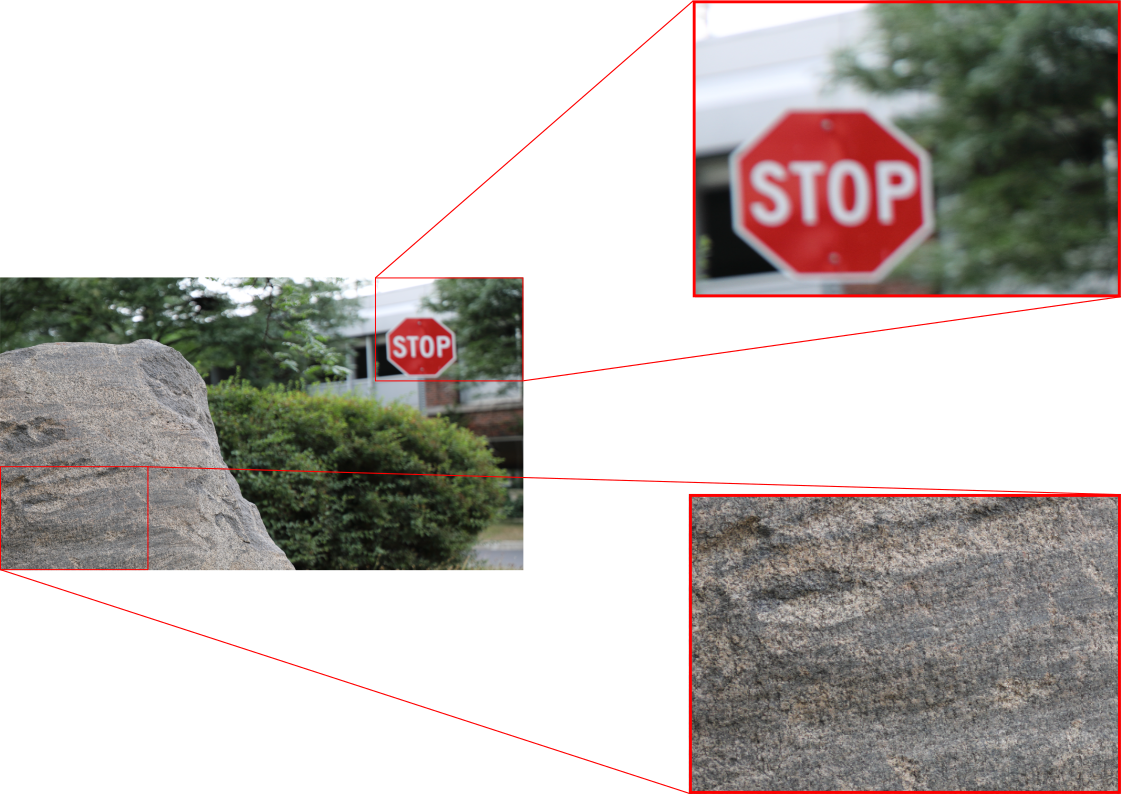
\includegraphics[width=0.6\textwidth]{images/Zoom1}
    \caption{Local enlarged view of an image}
    \label{fig:Zoom1}
\end{figure}

\par From the perspective of research paradigm, image focus detection usually
relies on local modeling rather than purely global modeling. This is because
focus state itself has obvious spatial non-uniformity, and image-level average
statistics are often not sufficient to accurately reflect the specific
locations of local edge diffusion, texture weakening, or high-frequency
information loss. For this reason, patch-based representation
\cite{Hou_2016_CVPR} has gradually become a common practice in this kind of
task. The image is first divided into local patches of fixed size, and then
each patch is treated as the basic analysis unit for sharpness evaluation or
supervised classification. This strategy can preserve local structural
features, and it is also convenient for organizing the subsequent processes of
feature extraction, label construction, model training, and visualizing the
projected-back results.

\par Existing related methods can be roughly divided into two categories. The
first category is traditional methods based on hand-crafted features
\cite{murphy2022pml}. These methods usually use gradient, edge, Laplacian
response, or high-frequency information in the frequency domain to describe
local clarity, and then combine classifiers such as support vector machines,
decision trees, or random forests for discrimination. Such methods are simple
to implement, relatively interpretable, and usually friendly to small or
medium-sized datasets. The second category is methods based on convolutional
neural networks (CNNs) \cite{lecun2002gradient,krizhevsky2012imagenet}. Their
main advantage is that they can automatically learn discriminative patterns
directly from pixels, and they often have stronger representation ability in
scenes with complex textures and nonlinear feature combinations. However, deep
models usually depend more on sufficient data support. Especially for
patch-level tasks, both the quality and quantity of training samples directly
affect model stability.

\par This thesis focuses exactly on this practical problem: in patch-based image
focus detection, when the available training data are limited and the cost of
manual patch-by-patch annotation is high, what are the respective advantages
and limitations of traditional machine learning methods and lightweight CNNs,
and what are their performance boundaries under a unified task definition. This
question has both engineering value and research significance, and it forms the
starting point of this work.

\section{Problem Formulation}

\par To organize image focus detection as a repeatable and comparable supervised
learning task, this thesis adopts a unified patch-based modeling framework
\cite{Hou_2016_CVPR}. For each input image, uniform preprocessing is first
performed, and then the image is divided into local patches. Each patch is
treated as the most basic analysis object. In this way, the spatial focus
distribution in the original image can be transformed into a local visual
classification problem that is easier to model, train, and compare.

\par Under this framework, image focus detection is no longer expressed only as
a subjective visual judgment problem, but is uniformly represented as a
standard supervised learning task \cite{murphy2022pml}. This thesis focuses on
the discrimination of focus states in different local regions, and further
compares the changes in model performance under different task settings, so as
to analyze the modeling characteristics of patch-level focus detection more
systematically.

\par Because manual annotation for each patch is costly, this thesis does not
use a labeling strategy that fully depends on manual annotation. Instead, it
designs an automatic labeling process \cite{5739529,1284395} to provide
consistent and repeatable supervisory signals for subsequent supervised
learning. At the same time, to reduce the interference of low-texture regions
on discrimination results, the thesis handles samples that are difficult to
classify stably during data organization and evaluation.

\par It should be emphasized that the automatic labeling mechanism and the
subsequent supervised classification are functionally separated. The former is
used to construct the labels required for training and evaluation, while the
latter is used to compare the discrimination ability of different models on the
same data basis. With this design, the thesis can analyze more clearly the
applicability and performance boundaries of different modeling methods under
the same task definition.

\section{Research Gap and Challenges}

\par Although there has already been substantial research on blur analysis,
sharpness evaluation, and local image classification, there are still several
issues worth further discussion for the patch-level image focus detection task
studied in this thesis, especially under limited data conditions.

\par First, deep learning methods perform strongly in many image tasks, but
their advantages are often built on relatively sufficient training data. When
the number of patch-level samples is limited and the labels do not come from
high-cost manual fine annotation, whether a CNN can stably learn effective
discriminative patterns and maintain generalization ability is not a conclusion
that can be assumed in advance. Second, although traditional machine learning
methods are usually easier to train and control under small-sample conditions,
their performance may be limited by the expressive ability of the input
representation. When facing samples with complex texture structures, weakened
edges, or ambiguous class boundaries, their classification ability may also be
unstable.

\par More importantly, existing studies often focus on optimizing only one kind
of method, while systematic comparisons between traditional methods and
lightweight CNNs under a unified data processing pipeline, unified label
system, and unified evaluation criteria are still lacking. For patch-based
image focus detection \cite{Hou_2016_CVPR}, it is still unclear how different
methods should be balanced in terms of accuracy, robustness, training cost, and
dependence on sample size.

\par In addition to the gap in model comparison, the task itself also faces
several direct challenges. The first is how to construct sufficiently
consistent and repeatable patch-level supervisory signals without relying on
manual patch-by-patch annotation. The second is how to organize the input,
training, and evaluation of traditional machine learning models
\cite{murphy2022pml} and CNNs under a unified pipeline, so that the comparison
is fair. The third is how to analyze the influence of sample size, class
imbalance handling, and binary versus three-class task settings on the final
results. These issues together form the core challenges that the research
design of this thesis aims to address.

\section{Research Motivation}

\par The motivation of this thesis comes from both engineering practice and
methodological research. From the engineering perspective, it is often
difficult to obtain large-scale and high-quality manual patch-level annotation
data in practical image focus analysis tasks, and computing resources may also
be limited. Under such conditions, complex deep models are not always the best
choice. Therefore, it is necessary to clarify the applicable boundaries of
different methods under low-sample conditions and provide a more operational
basis for subsequent system design.

\par From the research perspective, no unified conclusion has been formed on
the relative advantages of traditional machine learning methods and lightweight
CNNs in small-sample local visual classification tasks. Especially in the
patch-level focus detection scenario considered in this thesis, the
discrimination ability, stability, and applicable boundaries of different
methods under limited data conditions still need to be answered through
systematic comparison within a unified experimental framework.

\par Based on the above considerations, this thesis intends to study the
following core questions. First, can the automatic labeling mechanism provide
usable and relatively stable supervisory signals for subsequent patch-level
supervised learning? Second, under the same training set, validation set, and
evaluation metrics, how do traditional machine learning methods and lightweight
CNNs perform respectively? Third, when the task setting and training data
conditions change, what differences will appear in the performance trends and
applicable scenarios of different methods? Answers to these questions serve not
only practical method selection, but also help supplement empirical knowledge
in small-sample visual classification research.

\section{Objectives and Contributions}

\par Around the above research questions, this thesis takes patch-based image
focus detection \cite{Hou_2016_CVPR} as the target task, builds a unified
experimental pipeline, and systematically compares the performance of
traditional machine learning methods and lightweight CNNs. The main objectives
and contributions of this thesis can be summarized as follows:

\begin{itemize}
    \item To build a complete and unified experimental framework covering image
          preprocessing, patch division, automatic labeling, model training,
          validation and evaluation, and prediction visualization, so that the
          experimental process remains consistent and repeatable.

    \item To design a patch-level automatic labeling method that reduces the
          cost of manual annotation while providing a consistent and
          interpretable basis for label construction in supervised learning
          tasks.

    \item To systematically compare the classification performance of
          traditional machine learning methods \cite{murphy2022pml} and
          lightweight CNNs under low-sample conditions with unified data
          organization and evaluation criteria, and to analyze the differences
          between different modeling paradigms in accuracy, class recognition
          ability, robustness, and training complexity.

    \item To further examine the influence of sample size, class imbalance
          handling strategies, and binary versus three-class task settings on
          the results, so as to provide reference for method selection in image
          focus detection and similar small-sample local visual classification
          tasks.
\end{itemize}

\section{Overview of Research Approach}

\par From the perspective of the overall technical route, the method of this
thesis can be summarized into four stages. In the first stage, uniform
preprocessing is applied to the original images, and the images are divided
into a regular patch grid. In the second stage, automatic labels are
constructed based on local sharpness information. In the third stage,
traditional machine learning models and lightweight CNNs are trained under a
unified data representation. In the fourth stage, different methods are
systematically compared under unified evaluation criteria, and their
discrimination behavior is analyzed together with result visualization.

\par In terms of model setting, this thesis includes traditional machine
learning methods and lightweight CNNs in the same experimental framework and
conducts comparative experiments under different task settings and data
conditions. In this way, the thesis can observe more comprehensively the
applicable boundaries of different methods in the patch-based image focus
detection task.

\section{Organization of the Thesis}

\par The rest of this thesis is organized as follows. Chapter 2 introduces the
theoretical foundations related to this work, including the imaging degradation
mechanism of focus and blur, patch-based image representation, sharpness
features, traditional machine learning models, convolutional neural networks,
and learning characteristics under limited data conditions. It also provides
the main mathematical definitions and evaluation metrics used in the subsequent
experiments. Chapter 3 describes in detail the method design and implementation
process of this thesis, including image preprocessing, patch division,
automatic labeling rules, the training strategy of traditional models and
lightweight CNNs, and the overall comparative experimental design. The
following chapters present the experimental results based on the above theory
and methods, analyze the performance of different models under different task
settings, and finally summarize the whole work and the main conclusions of this
thesis.
